\documentclass{beamer}
\usepackage{amsfonts}
\usepackage{amsmath}
\usepackage{amssymb}
\usepackage{amsthm}
\usepackage{enumerate}
\usepackage{graphicx}
\usepackage{layout}
\usepackage{mathrsfs}
\usepackage{fancyhdr}
\usepackage{subfigure}
\usepackage{tcolorbox}
\usepackage{tikz-cd}
\usepackage{ctex}
\usepackage{color}
%\usepackage{fontspec}

\usepackage{mathtools}
\usepackage{float}
\usepackage{bm}
\usepackage{booktabs}
\usetheme{Darmstadt}
\usecolortheme{dolphin}

%\setmainfont{Latin Modern Roman:style=6 Bold,Bold}
\newcommand{\dif}{\mathrm{d}}
\newtheorem{thm}{Theorem}
\begin{document}
\title{Programming of 3D Boolean Algebra on Yin Set}
\author{Yan Tan}
\date{\today}
\maketitle

\begin{frame}
  \frametitle{Contents}
  \tableofcontents
\end{frame}

\section{Mathmatical Concept}

\begin{frame}
  \frametitle{What?}
  \begin{itemize}

    
  \item A Yin set  $\mathbb{Y} \subseteq \mathbb{R}^3$ is a \textcolor[rgb]{1,0,0}{regular open} \textcolor[rgb]{1,0,1}{semianalytic} set whose \textcolor[rgb]{0,0,1}{boundary is bounded}. The class of all such Yin sets form the Yin space $\mathbb{Y}$.
  \item   Boolean algebra
    \begin{itemize}
    \item $\widehat{0}$ and $\widehat{1}$ respectively get $ \emptyset$ and $\mathbb{R}^3$
    \item Complementation $\prime$.
    \item Meet operation $\wedge$ .
    \item Join operation $\vee$ can be realized by $\prime$ and $\wedge$.
    
    \end{itemize}
 % \item  Simple and efficient Boolean algorithms
  \end{itemize}
     \begin{figure}[h]
      \centering
     % \includegraphics[scale=0.25]{panda.png}
    \end{figure}
\end{frame}

%\begin{frame}
%  \frametitle{Why?}
%  \begin{itemize}
%  \item Fluid modeling for multiphase flows in 3D space.
%  \end{itemize}
%\end{frame}

\begin{frame}
  \frametitle{How?}
  
  \begin{itemize}
   % \item Yin space $\mathbb{Y}$ represent 3D fluid.
  \item Represent Yin sets $\mathbb{Y}$ by their oriented boundary $\mathbb{J}$.
%    \begin{equation}\notag
%      \mathcal{Y} = \cup_j^{\perp \perp}\cap_i \text{int}(\gamma_{j, i})
%    \end{equation}
\item The boundary of every connected component of a Yin set is an orientable compact surface.
\item A partial order exists between these surfaces like the inclusion relation in 2D.
%  \item Every connected subset of Yin set whose boundary has a relation like hassmap.
  \item $\mathbb{J}$ can be approximately represented by a set of oriented triangles $\mathbb{T}$. 
  \item An isomorphism $\rho$ between $\mathbb{T}$  and $\mathbb{Y}$
    \begin{itemize}
    \item Reduce a 3-dimensional problem into 2-dimensional
    \end{itemize}
    
  % \item Conjugation:
  %   \begin{equation*}
  %     \rho \circ b \circ \rho^{-1}
  %   \end{equation*}
  \end{itemize}
\end{frame}

\section{C++ implementation}

\begin{frame}
  \frametitle{Translating Mathematic Concepts to Class}
  \begin{itemize}
  \item Point $\to$ Class \textbf{Point}
  \item Vector $\to$ Class \textbf{Direction}
  \item Straight Line $\to$ Class \textbf{Line}
  \item Segment $\to$ Class \textbf{Segment} : public \textbf{Line}  
  \item Flat $\to$ Class \textbf{Flat}
  \item Planar $\to$ Class \textbf{Planar} : public \textbf{Flat}
  \item Oriented and connected face formed by a set of triangles $\to$ Class \textbf{Face}
  \item Yin set's boundary $\to$ Class \textbf{Spadjor}
  \item Yin set $\to$ Class \textbf{Object}
   % \item To make our implementation more robust, a tolerance (controlled by the user) is added whenever possible
  %\item And some class contain tolerance, hassmap relation and operations that are used to compute triangles intersection, determine a triangle if still is part of Yin set's boundary after meet operation and so on.
  \end{itemize}
\end{frame}

\begin{frame}
  \frametitle{Relations Between These Classes}
  "has a" :
  \begin{itemize}
  \item \textbf{Segment} has two \textbf{Point}s that are its endpoint.  
  \item \textbf{Planar} has at least three \textbf{Segment}s as its boundary.
  \item \textbf{Face} has at least four \textbf{Planar}s.
  \item \textbf{Spadjor} has at least one \textbf{Face}.  
  %\item Jordan curve $\Longleftrightarrow$ \textbf{Polygon} (``is-a'' \textbf{SimplePath})
  \end{itemize}

  "is a":
  \begin{itemize}
  \item \textbf{Segment} is a \textbf{Line} and has two \textbf{Point}s as endpoints.
   

    
  \item \textbf{Planar} is a \textbf{Flat} contains some \textbf{Segment}s as edges.
  \end{itemize}
\end{frame}

\begin{frame}
  %\frametitle{UNL Class Diagram}
  % \begin{thm}
  %   Any realizable spadjor $\mathcal{J}$ can be uniquely expressed as
  %   \begin{equation}
  %     \mathcal{J} = \cup_{i=1}^n\mathcal{J}_i^+ \cup \mathcal{J}^{-}
  %   \end{equation}
  % \end{thm}
  \begin{figure}[htbp]
  	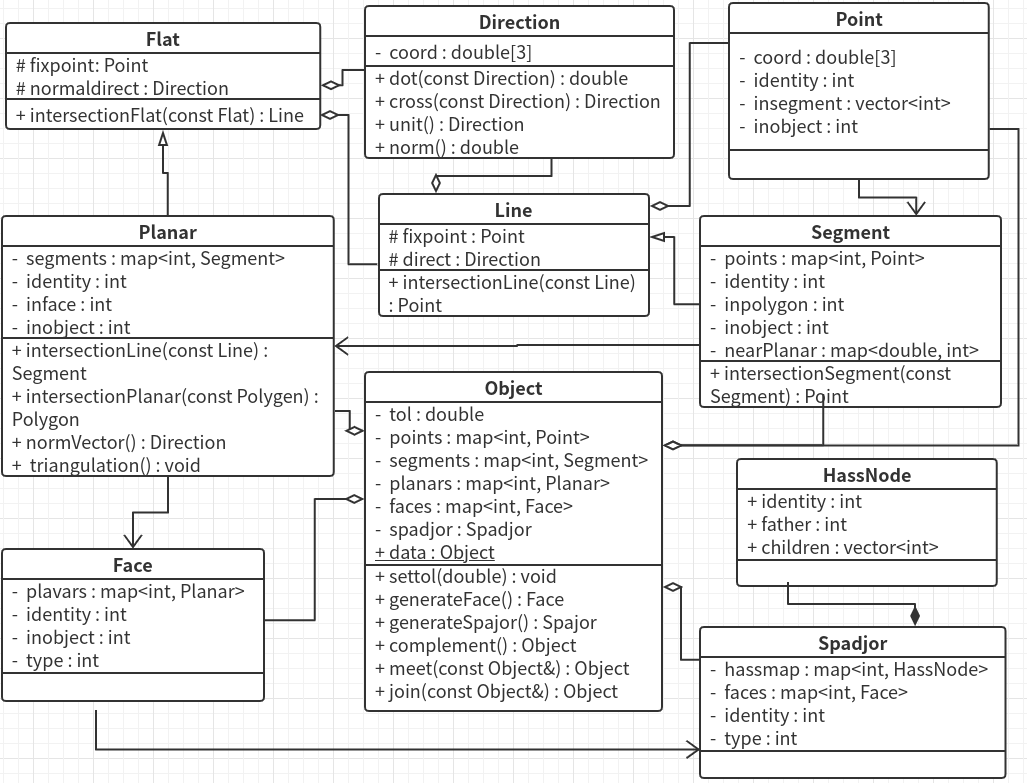
\includegraphics[scale=0.295]{UMLclass.png}
%    \centering
%    \subfigure[a Yin set with four connected components]{
%       % \includegraphics[scale=0.2]{simpleYinSet.png}
%      }
%      \quad
%      \subfigure[its corresponding Hasse diagram]{
%        %\includegraphics[scale=0.2]{HasseDiagram.png}
%      }
  \end{figure}
%  \begin{itemize}
%
%    
%  \item Inclusion relation of Jordan curves
%  \item Decomposition into atom spadjors (Lemma 3.18)
%
%    
%  \item Topological information
%  \end{itemize}
\end{frame}

\begin{frame}
  \frametitle{How to Realize Boolean Operations}
  \begin{itemize}
  \item Complementation $\prime$ can be accomplished by changing orientation of boundary of Yin sets $\mathbb{Y}$,
  we can do that by change planar's orientation. 

    
  \item Meet operation $\wedge$ can be done by taking the following five operations.
    \begin{itemize}
    	\item[1] Computing triangles intersection generates some segments and some triangles change into some planars.
    	\item[2] Do triangulation for planar.
    	\item[3] Determine triangles if still part of the Yin set's boundary after meet operation.
    	%\item Do trianglulation for polygon.
    	\item[4] Pasting every triangles to some faces represent Yin set's boundary.
    	\item[5] Create a new hassmap represent faces' inclusion relation.
    \end{itemize}
   \end{itemize}


    
%  \item Generate a realizable spadjor
%    $\Longleftrightarrow$ \textbf{SpadjorGenerator}
%    \begin{itemize}
%    \item either through an array of \textbf{Polygon}s
%    \item or through an input file
%      \item a protected method: void buildHasse(const
%        vector$\langle$\textbf{Polygon}$\rangle$ \&,
%        vector$\langle$\textbf{Node}$\rangle$ \&) const;
%    \end{itemize}
%
%  \item
%    \textbf{RealizableSpadjor} consists of simple ``get'' functions.
%    \begin{itemize}
%    \item Betti numbers
%    \item Hasse diagram
%      \item ...
%    \end{itemize}
%    % \begin{itemize}
%    % \item int numConnectedcomponents() const;
%      
%    % \item int numHoles(int i) const;
%      
%    % \item string HasseDiagram() const;
%      
%    % \item bool isBounded() const;
%      
%    % \item ...
%    % \end{itemize}
%  \end{itemize}
\end{frame}

\begin{frame}
  \frametitle{Pasting operation}
  \begin{itemize}
  \item Using a Stack st.
  \begin{itemize}
  \item st's element is Planar that have finished triangulation. So it contains triangles.
  \end{itemize}
\item St is empty at first. Choose a triangle hasn't been pasted push in and save it in a empty map<int, Planar> m.
  \begin{itemize}
  \item[1] pop the triangle t in the Top of st. 
  \item[2] then find triangles that share an edge with t if it hasn't been pasted and should be pasted with t. 
  \item[3] if triangle t1 should be pasted, push t1 into st and save it in the map m.
  \item[4] if no triangles should be pasted. Back to first step and continue.
  \item[5] if st becomes empty again, using the map m create a new face.Then break the loop.
  \end{itemize}
  
%\item How to determine a triangle whether should be pasted with t.
%  \begin{itemize}
%  \item choose a edge e of t.
%  \item fix e, rotate t in the opposite direction to the normal vector of t until find the first triangle t1 that has edge e and has normal vector that is opposite to t`s.
%  \end{itemize}
%  

  \end{itemize}
\end{frame}

\begin{frame}
  \begin{itemize}
  \item How to determine whether a triangle should be pasted with t.
  \begin{itemize}
  	\item choose an edge e of t.
  	\item fix e, rotate t in the opposite direction to the normal vector of t until finding the first triangle t1 that has edge e and has normal vector that is opposite to t's. t1 is the only triangle share edge e should be pasted with t.
  \end{itemize}
  \end{itemize}
\begin{figure}
	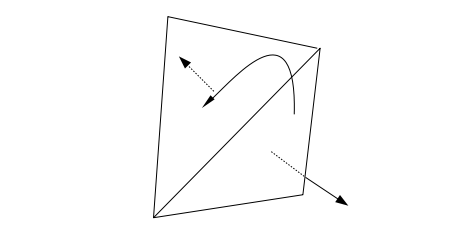
\includegraphics[scale=0.4]{past.png}
\end{figure}
   \textcolor[rgb]{1,0,0}{regular open} \textcolor[rgb]{1,0,1}{semianalytic} \textcolor[rgb]{0,0,1}{boundary is bounded}
\end{frame}

%\begin{frame}
%  \frametitle{Usage}
%       \begin{figure}[h]
%      \centering
%    %  \includegraphics[scale=0.29]{usage.png}
%    \end{figure}
%\end{frame}

\section{Test}

\begin{frame}
  \frametitle{Test Work}
  Test data : 
  \begin{itemize}
  \item spheres, torus, n-ple torus. 
    
  \item two cylinders coincide in a line.
    
  \item two tetrahedrons have a triangle planar contain another or coincide in a point.

  \end{itemize}
  Test way : 
  \begin{itemize}
  	\item input data in Obj format.
  	\item output data in Obj format.
  	\item render with ray tracing.
  \end{itemize}
\end{frame}

%\begin{frame}
%	\frametitle{Some Faults}
%	\begin{itemize}
%		\item programing through geometric intuition.
%		\item without mathematical proof of the correctness
%		\item haven't considered the effectiveness.
%		\item lack of test data. 
%	\end{itemize}
%\end{frame}

\end{document}
